%package list
\documentclass{article}
\usepackage[top=3cm, bottom=3cm, outer=3cm, inner=3cm]{geometry}
\usepackage{multicol}
\usepackage{graphicx}
\usepackage{url}
%\usepackage{cite}
\usepackage{hyperref}
\usepackage{array}
%\usepackage{multicol}
\newcolumntype{x}[1]{>{\centering\arraybackslash\hspace{0pt}}p{#1}}
\usepackage{natbib}
\usepackage{pdfpages}
\usepackage{multirow}
\usepackage[normalem]{ulem}
\useunder{\uline}{\ul}{}
\usepackage{svg}
\usepackage{xcolor}
\usepackage{listings}
\lstdefinestyle{ascii-tree}{
    literate={├}{|}1 {─}{--}1 {└}{+}1 
  }
\lstset{basicstyle=\ttfamily,
  showstringspaces=false,
  commentstyle=\color{red},
  keywordstyle=\color{blue}
}
%\usepackage{booktabs}
\usepackage{caption}
\usepackage{subcaption}
\usepackage{float}
\usepackage{array}

\newcolumntype{M}[1]{>{\centering\arraybackslash}m{#1}}
\newcolumntype{N}{@{}m{0pt}@{}}


%%%%%%%%%%%%%%%%%%%%%%%%%%%%%%%%%%%%%%%%%%%%%%%%%%%%%%%%%%%%%%%%%%%%%%%%%%%%
%%%%%%%%%%%%%%%%%%%%%%%%%%%%%%%%%%%%%%%%%%%%%%%%%%%%%%%%%%%%%%%%%%%%%%%%%%%%
\newcommand{\itemEmail}{phidalgo@unsa.edu.pe}
\newcommand{\itemStudent}{Paulo Andre Hidalgo Chinchay}
\newcommand{\itemCourse}{Programación web 2}
\newcommand{\itemCourseCode}{20223011}
\newcommand{\itemSemester}{III}
\newcommand{\itemUniversity}{Universidad Nacional de San Agustín de Arequipa}
\newcommand{\itemFaculty}{Facultad de Ingeniería de Producción y Servicios}
\newcommand{\itemDepartment}{Departamento Académico de Ingeniería de Sistemas e Informática}
\newcommand{\itemSchool}{Escuela Profesional de Ingeniería de Sistemas}
\newcommand{\itemAcademic}{2023 - A}
\newcommand{\itemInput}{Del 2 Junio 2023}
\newcommand{\itemOutput}{Al 9 Junio 2023}
\newcommand{\itemPracticeNumber}{04}
\newcommand{\itemTheme}{Python}
%%%%%%%%%%%%%%%%%%%%%%%%%%%%%%%%%%%%%%%%%%%%%%%%%%%%%%%%%%%%%%%%%%%%%%%%%%%%
%%%%%%%%%%%%%%%%%%%%%%%%%%%%%%%%%%%%%%%%%%%%%%%%%%%%%%%%%%%%%%%%%%%%%%%%%%%%

\usepackage[english,spanish]{babel}
\usepackage[utf8]{inputenc}
\AtBeginDocument{\selectlanguage{spanish}}
\renewcommand{\figurename}{Figura}
\renewcommand{\refname}{Referencias}
\renewcommand{\tablename}{Tabla} %esto no funciona cuando se usa babel
\AtBeginDocument{%
	\renewcommand\tablename{Tabla}
}

\usepackage{fancyhdr}
\pagestyle{fancy}
\fancyhf{}
\setlength{\headheight}{30pt}
\renewcommand{\headrulewidth}{1pt}
\renewcommand{\footrulewidth}{1pt}
\fancyhead[L]{\raisebox{-0.2\height}{
\includegraphics[width=3cm]{img/logo_episunsa.png}}}
\fancyhead[C]{\fontsize{7}{7}\selectfont	\itemUniversity \\ \itemFaculty \\ \itemDepartment \\ \itemSchool \\ \textbf{\itemCourse}}
\fancyhead[R]{\raisebox{-0.2\height}{
\includegraphics[width=1.2cm]{img/logo_abet}}}
\fancyfoot[L]{Estudiante Paulo Hidalgo Chinchay}
\fancyfoot[C]{\itemCourse}
\fancyfoot[R]{Página \thepage}

% para el codigo fuente
\usepackage{listings}
\usepackage{color, colortbl}
\definecolor{dkgreen}{rgb}{0,0.6,0}
\definecolor{gray}{rgb}{0.5,0.5,0.5}
\definecolor{mauve}{rgb}{0.58,0,0.82}
\definecolor{codebackground}{rgb}{0.95, 0.95, 0.92}
\definecolor{tablebackground}{rgb}{0.8, 0, 0}

\lstset{frame=tb,
	language=bash,
	aboveskip=3mm,
	belowskip=3mm,
	showstringspaces=false,
	columns=flexible,
	basicstyle={\small\ttfamily},
	numbers=none,
	numberstyle=\tiny\color{gray},
	keywordstyle=\color{blue},
	commentstyle=\color{dkgreen},
	stringstyle=\color{mauve},
	breaklines=true,
	breakatwhitespace=true,
	tabsize=3,
	backgroundcolor= \color{codebackground},
}

\begin{document}
	
	\vspace*{10px}
	
	\begin{center}	
		\fontsize{17}{17} \textbf{ Informe de Laboratorio \itemPracticeNumber}
	\end{center}
	\centerline{\textbf{\Large Tema: \itemTheme}}
	%\vspace*{0.5cm}	

	\begin{flushright}
		\begin{tabular}{|M{2.5cm}|N|}
			\hline 
			\rowcolor{tablebackground}
			\color{white} \textbf{Nota}  \\
			\hline 
			     \\[30pt]
			\hline 			
		\end{tabular}
	\end{flushright}	

	\begin{table}[H]
		\begin{tabular}{|x{4.7cm}|x{4.8cm}|x{4.8cm}|}
			\hline 
			\rowcolor{tablebackground}
			\color{white} \textbf{Estudiante} & \color{white}\textbf{Escuela}  & \color{white}\textbf{Asignatura}   \\
			\hline 
			{\itemStudent \par \itemEmail} & \itemSchool & {\itemCourse \par Semestre: \itemSemester \par Código: \itemCourseCode}     \\
			\hline 			
		\end{tabular}
	\end{table}		
	
	\begin{table}[H]
		\begin{tabular}{|x{4.7cm}|x{4.8cm}|x{4.8cm}|}
			\hline 
			\rowcolor{tablebackground}
			\color{white}\textbf{Laboratorio} & \color{white}\textbf{Tema}  & \color{white}\textbf{Duración}   \\
			\hline 
			\itemPracticeNumber & \itemTheme & 04 horas   \\
			\hline 
		\end{tabular}
	\end{table}
	
	\begin{table}[H]
		\begin{tabular}{|x{4.7cm}|x{4.8cm}|x{4.8cm}|}
			\hline 
			\rowcolor{tablebackground}
			\color{white}\textbf{Semestre académico} & \color{white}\textbf{Fecha de inicio}  & \color{white}\textbf{Fecha de entrega}   \\
			\hline 
			\itemAcademic & \itemInput &  \itemOutput  \\
			\hline 
		\end{tabular}
	\end{table}
	
	\section{Tarea}
	\begin{itemize}		
		\item  Implemente los métodos de la clase Picture. Se recomienda que implemente la clase picture
		por etapas, probando realizar los dibujos que se muestran en la siguiente preguntas.
		\subitem Usando  únicamente los métodos de los objetos de la clase Picture dibuje las siguientes
		figuras (invoque a draw):
		\subitem Para resolver los siguientes ejercicios solo está permitido usar ciclos, condicionales, definición
		de listas por comprensión, sublistas, map, join, (+), lambda, zip, append, pop, range.
	\end{itemize}
		
	\section{Equipos, materiales y temas utilizados}
	\begin{itemize}
		\item Sistema Operativo Ubuntu GNU Linux 23 lunar 64 bits Kernell 6.2.
		\item Sistema Operativo Windows 11 pro versión 22H2 de 64 bits.
		\item VIM 9.0.
		\item Git 2.39.2.
		\item Visual Studio Code 1.78.2.
		\item Cuenta en GitHub con el correo institucional.
		\item NodeJS 18.1.0
		\item Clases de 1 a 31 del curso de Udemy "Python Practicando. Desde 0 hasta Desarrollador en Python"
		\item \url{https://www.udemy.com/share/101sJC3@xod_U1pjR_efxIhsxPzAUuEnE3ok_9rlPTHMowoqaob1g4YfN7M-j7alvT0_tbf4Vw==/}
		\item Uso de append por w3schools
		\item \item \url{https://www.w3schools.com/python/ref_list_append.asp}
	\end{itemize}
	
	\section{URL de Repositorio Github}
	\begin{itemize}
		\item URL del Repositorio GitHub para clonar o recuperar.
		\item \url{https://github.com/PauloUNSA/pw2-lab-c-23a.git}
		\item URL para el laboratorio 03 en el Repositorio GitHub.
		\item \url{https://github.com/PauloUNSA/pw2-lab-c-23a/tree/main/lab4}
	\end{itemize}
	
	\section{Configurar espacio de trabajo}
	\begin{itemize}	
		\item El archivo picture.py es la clase picture que contiene algunos metodos ya desarrollados
		los otros se desarrollaran en y explicaran aqui.
		\item Para poder ejecutar todos los ejercicios se tuvo que instalar la liberia Pygame
		con el siguiente comando.
	\end{itemize}	
	\begin{lstlisting}[language=bash,caption={Instalar libreria Pygame}][H]
		$ pip install pygame
	\end{lstlisting}
	\section{Ejercicios}
	%%%%%%%%%%%%%%%%%%%%%%%%%%%%%
	\subsection{Primer ejercicio}
	\begin{itemize}	
		\item Se tuvieron que implementar las funciones negative, join y under. 
		En el codigo se detalla lo que hacen.
	\end{itemize}
	\lstinputlisting[language=Python, caption={Picture version 1},numbers=left,]{src/pic01.py}
	Para implementar el negativo se cambia el color de cada carácter, a excepción del espacio
	ya que este no tiene inverso con doble for(1 anidado). Juntando estos caracteres
	por medio en una cadena y despues juntando esta cadena al nuevo arreglo 
	con el metodo append.
	\lstinputlisting[language=Python, caption={Ejercicio 2 a},numbers=left,]{src/e2a.py}
	Para poder hacer que se dibuje como se mostrara el la figura de abajo se tuvo de juntar un caballo
	blanco con uno negro en la primera fila; para ello se utilizo join y negative. Para la segunda
	fila se necesito saltar a la siguiente fila por lo que se utilizo el metodo under.
	\begin{figure}[H]
		\centering
		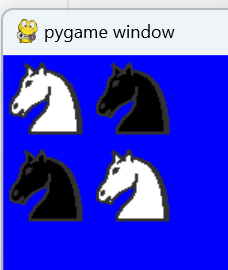
\includegraphics[width=0.4\textwidth,keepaspectratio]{img/e2a.png}
		\caption{Ejecución exitosa ejercicio 2 a}
	\end{figure}
	%%%%%%%%%%%%%%%%%%%%%%%%%%%%%
	\subsection{Segundo ejercicio}
	\begin{itemize}	
		\item Se tuvieron que implementar la función horizontalMirror Y verticalMirror. 
		Se detalla lo que hace a continuación.
	\end{itemize}
	\lstinputlisting[language=Python, caption={Picture version 2},numbers=left,]{src/pic02.py}
	Para no gastar espacio de más a partir de aqui solo se coloco las funciones las funciones de clase
	y el métodos horizontalMirror y verticalMirror. El método horizontalMirror solo 
	devuelve el arreglo al revés, el 1er elemento al ultimo y el ultimo al 1ro. verticalMirror
	tiene que entrar en cadena y ordenarla al revés, juntándola en el arreglo vertical y 
	retornándola como Picture.
	\lstinputlisting[language=Python, caption={Ejercicio 2 b},numbers=left,]{src/e2b.py}
	La 1ra fila se hace de igual forma que en el 1er ejercicio sin embargo para la fila de abajo 
	se agregar .verticalMirror a ambos caballos para invertir verticalmente las figuras.
	\begin{figure}[H]
		\centering
		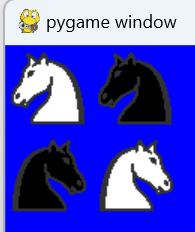
\includegraphics[width=0.3\textwidth,keepaspectratio]{img/e2b.png}
		\caption{Ejecución exitosa ejercicio 2 b}
	\end{figure}
	%%%%%%%%%%%%%%%%%%%%%%%%%%%%%
	\subsection{Tercer ejercicio}
	\begin{itemize}	
		\item No se tuvo que implementar método adicionar
	\end{itemize}
	\lstinputlisting[language=Python, caption={Ejercicio 2 c},numbers=left,]{src/e2c.py}
	Una sola final de 4 reinas del mismo color con el método join.
	\begin{figure}[H]
		\centering
		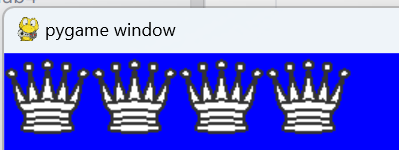
\includegraphics[width=0.4\textwidth,keepaspectratio]{img/e2c.png}
		\caption{Ejecución exitosa ejercicio 2 c}
	\end{figure}
	%%%%%%%%%%%%%%%%%%%%%%%%%%%%%
	\subsection{Cuarto ejercicio}
	\begin{itemize}	
		\item Se tuvieron que implementar la función horizontalRepeat Y verticalRepeat. 
		Se detalla lo que hace a continuación.
	\end{itemize}
	\lstinputlisting[language=Python, caption={Picture version 3},numbers=left,]{src/pic03.py}
	El método horizontalRepeat multiplica n veces abajo el arreglo y verticalMirror
	tiene la misma lógica pero en este caso hacia la derecha.
	\lstinputlisting[language=Python, caption={Ejercicio 2 d},numbers=left,]{src/e2d.py}
	1 sola fila de 8 casillas intercaladas, primero clara y después oscura. Para ello se referecian 2 y despues con 
	el método verticalRepeat se repite 4 veces.
	\begin{figure}[H]
		\centering
		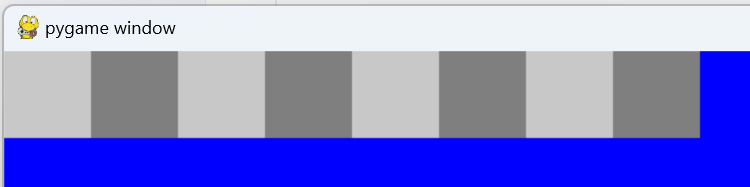
\includegraphics[width=0.3\textwidth,keepaspectratio]{img/e2d.png}
		\caption{Ejecución exitosa ejercicio 2 d}
	\end{figure}
	%%%%%%%%%%%%%%%%%%%%%%%%%%%%%
	\subsection{Quinto ejercicio}
	\begin{itemize}	
		\item No se implemento método adicional.
	\end{itemize}
	\lstinputlisting[language=Python, caption={Ejercicio 2 e},numbers=left,]{src/e2e.py}
	Igual que el 4to sino que las casillas van al revés, oscuras después claras
	\begin{figure}[H]
		\centering
		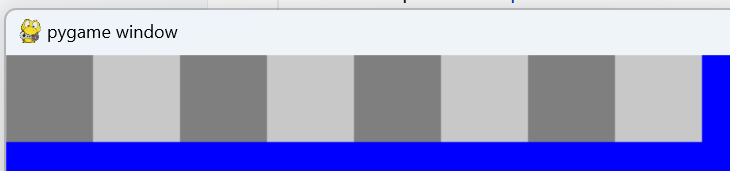
\includegraphics[width=0.3\textwidth,keepaspectratio]{img/e2e.png}
		\caption{Ejecución exitosa ejercicio 2 e}
	\end{figure}
	%%%%%%%%%%%%%%%%%%%%%%%%%%%%%
	\subsection{Sexto ejercicio}
	\begin{itemize}	
		\item No se implemento método adicional.
	\end{itemize}
	\lstinputlisting[language=Python, caption={Ejercicio 2 f},numbers=left,]{src/e2f.py}
	Se baso en el 4to y 5to ejercicio donde se juntaron ambos con el método under 
	y se duplico con el método horizontalRepeat.
	\begin{figure}[H]
		\centering
		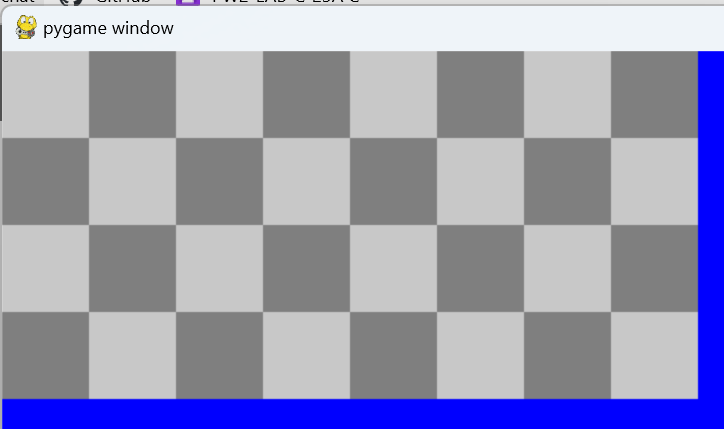
\includegraphics[width=0.3\textwidth,keepaspectratio]{img/e2f.png}
		\caption{Ejecución exitosa ejercicio 2 f}
	\end{figure}
	%%%%%%%%%%%%%%%%%%%%%%%%%%%%%
	\subsection{Ultimo ejercicio}
	\begin{itemize}	
		\item Se implemento el método up.
	\end{itemize}
	\lstinputlisting[language=Python, caption={Picture version 4},numbers=left,]{src/pic04.py}
	El método up hace que se sobreponga la figura recibida como argumento. Donde primero se 
	valida si el carácter de la figura que ira encima no sea un espacio, en caso se cumpla
	ira el carácter de la figura de encima sino ira el de la figura de abajo.
	\lstinputlisting[language=Python, caption={Ejercicio 2 d},numbers=left,]{src/e2g.py}
	Se reutilizo el codigo del 6to ejercicio para medio. y de subdividio en derecha, izquiera y centro
	para la fila principal, donde van las torres alfiles, caballos, reina y rey. 
	Se junto todo esto en filaAbajo ya que era donde iban los blancos. Y para filaArriba
	se añadio negative. Los peones solo eran una fila de casilla clara y oscura con peones encima.
	Quedando las partes superior que era igual a filaArriba concatenada con pNegros
	(los peones neegros) y para la parte inferior, filaAbajo concatenada con peonesBlancos.
	finalmente al draw se le paso el argumento superio.under(medio).under(inferior) quedando asi.
	\begin{figure}[H]
		\centering
		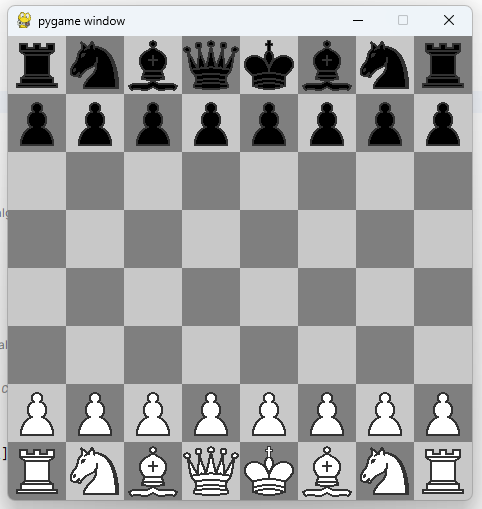
\includegraphics[width=0.5\textwidth,keepaspectratio]{img/e2g.png}
		\caption{Ejecución exitosa ejercicio 2 g}
	\end{figure}
	%%%%%%%%%%%%%%%%%%%%%%%%%%%%%
	\subsection{Estructura de laboratorio 04}
	\begin{itemize}	
		\item El contenido que se entrega en este laboratorio es el siguiente:
	\end{itemize}
	
\begin{lstlisting}[style=ascii-tree]
	//se omitieron las subcarpetas y archivos de node_modules al ocupar las de 500 lineas de espacio
	C:\USERS\PAULO\PW2-LAB-C-23A\LAB3
	|	├───express
	|   |   estilo.css
	|   |   index.html
	|   |   index.js
	|   |   package-lock.json
	|   |   package.json
	|   |   script.js
	|   |   
	|   ├───agenda
	|   ├───eventos
	|   ├───node_modules
	|   |   |   *
	|   |
	|   └───priv
	|           poema.txt
	|
	└───latex
		|   lab3_paulo-hidalgo.tex
		|	lab3_paulo-hidalgo.pdf
		|
		├───build
		|       lab3_paulo-hidalgo.aux
		|       lab3_paulo-hidalgo.fdb_latexmk
		|       lab3_paulo-hidalgo.fls
		|       lab3_paulo-hidalgo.log
		|       lab3_paulo-hidalgo.out
		|       lab3_paulo-hidalgo.pdf
		|       lab3_paulo-hidalgo.synctex(busy)
		|
		├───img
		|       crea-evento.png
		|       eliminar.png
		|       l-eventos.png
		|       localhost01.png
		|       localhost02.png
		|       localhost03.png
		|       localhost_agenda.png
		|       logo_abet.png
		|       logo_episunsa.png
		|       logo_unsa.jpg
		|       Segundo-commit.png
		|       ultimo-commit.png
		|       ver-eventos01.png
		|       ver-eventos02.png
		|
		└───src
				css01.css
				index01.html
				index02.html
				index03.html
				indexjs01.js
				indexjs02.js
				indexjs03.js
				script.js
\end{lstlisting}
\subsection{Pregunta: En el Ejemplo Hola Mundo con NodeJS. ¿Qué pasó con la línea: Content type ...?}
\begin{itemize}
	\item No esta debido a que no es necesario ya que devuelve una respuesta en JSON, que después
	es tomada por el cliente e insertada en un div de html ya existente.
\end{itemize}
	\clearpage
	\section{\textcolor{red}{Rúbricas}}

	\subsection{\textcolor{red}{Rúbrica para el contenido del Informe y demostración}}
	\begin{itemize}			
		\item El alumno debe marcar o dejar en blanco en celdas de la columna \textbf{Checklist} si cumplio con el ítem correspondiente.
		\item Si un alumno supera la fecha de entrega,  su calificación será sobre la nota mínima aprobada, siempre y cuando cumpla con todos lo items.
		\item El alumno debe autocalificarse en la columna \textbf{Estudiante} de acuerdo a la siguiente tabla:
	
		\begin{table}[ht]
			\caption{Niveles de desempeño}
			\begin{center}
			\begin{tabular}{ccccc}
    			\hline
    			 & \multicolumn{4}{c}{Nivel}\\
    			\cline{1-5}
    			\textbf{Puntos} & Insatisfactorio 25\%& En Proceso 50\% & Satisfactorio 75\% & Sobresaliente 100\%\\
    			\textbf{2.0}&0.5&1.0&1.5&2.0\\
    			\textbf{4.0}&1.0&2.0&3.0&4.0\\
    		\hline
			\end{tabular}
		\end{center}
	\end{table}	
	
	\end{itemize}
	
	\begin{table}[H]
		\caption{Rúbrica para contenido del Informe y demostración}
		\setlength{\tabcolsep}{0.5em} % for the horizontal padding
		{\renewcommand{\arraystretch}{1.5}% for the vertical padding
		%\begin{center}
		\begin{tabular}{|p{2.7cm}|p{7cm}|x{1.3cm}|p{1.2cm}|p{1.5cm}|p{1.1cm}|}
			\hline
    		\multicolumn{2}{|c|}{Contenido y demostración} & Puntos & Checklist & Estudiante & Profesor\\
			\hline
			\textbf{1. GitHub} & Hay enlace URL activo del directorio para el  laboratorio hacia su repositorio GitHub con código fuente terminado y fácil de revisar. &2 &X &2 & \\ 
			\hline
			\textbf{2. Commits} &  Hay capturas de pantalla de los commits más importantes con sus explicaciones detalladas. (El profesor puede preguntar para refrendar calificación). &4 &X &4 & \\ 
			\hline 
			\textbf{3. Código fuente} &  Hay porciones de código fuente importantes con numeración y explicaciones detalladas de sus funciones. &2 &X &2 & \\ 
			\hline 
			\textbf{4. Ejecución} & Se incluyen ejecuciones/pruebas del código fuente  explicadas gradualmente. &2 &X &2 & \\ 
			\hline			
			\textbf{5. Pregunta} & Se responde con completitud a la pregunta formulada en la tarea.  (El profesor puede preguntar para refrendar calificación).  &2 &X &2 & \\ 
			\hline	
			\textbf{6. Fechas} & Las fechas de modificación del código fuente estan dentro de los plazos de fecha de entrega establecidos. &2 &X &2 & \\ 
			\hline 
			\textbf{7. Ortografía} & El documento no muestra errores ortográficos. &2 &X &2 & \\ 
			\hline 
			\textbf{8. Madurez} & El Informe muestra de manera general una evolución de la madurez del código fuente,  explicaciones puntuales pero precisas y un acabado impecable.   (El profesor puede preguntar para refrendar calificación).  &4 &X &4 & \\ 
			\hline
			\multicolumn{2}{|c|}{\textbf{Total}} &20 & &20 & \\ 
			\hline
		\end{tabular}
		%\end{center}
		%\label{tab:multicol}
		}
	\end{table}
	
\clearpage

\section{Referencias}
\begin{itemize}			
	\item \url{https://github.com/rescobedoq/pw2/tree/main/labs/lab03}
	\item \url{https://www.w3schools.com/nodejs/nodejs_filesystem.asp}
\end{itemize}				
\end{document}